\documentclass[12pt]{book}
\usepackage{graphicx}
\usepackage{subfig} % make it possible to include more than one captioned figure/table in a single float
\usepackage[utf8]{inputenc}
\usepackage{hyperref}
\usepackage[intlimits]{amsmath}
\usepackage{amssymb}
\setlength{\oddsidemargin}{15.5pt} 
\setlength{\evensidemargin}{15.5pt}
\pretolerance=2000
\tolerance=3000
\renewcommand{\figurename}{Figura}
\renewcommand{\chaptername}{Cap\'{i}tulo}
\renewcommand{\contentsname}{\'{I}ndice}
\renewcommand{\tablename}{Tabla}
\renewcommand{\bibname}{Bibliograf\'{i}a}
\renewcommand{\appendixname}{Ap\'endices}


\title{Sistema autogravitante con simetría esférica y distribución exponencial de masa}
\date{}
\begin{document}
\section*{Nociones teóricas}

Para una distribución de masa $\rho$

\begin{description}
\item De la ley de Newton la fuerza gravitatoria ejercitada en el punto x es:  $F(x) = G \int{\frac{x\prime - x}{|x\prime - x|^3}\rho(x\prime)d^3x} $ y despues de hacer cálculos llegamos a $ \nabla F(x) = -4\pi G \rho(x) $
\item Definimos el potencial gravitatorio $\Phi(x) = -G \int{\frac{\rho(x\prime)}{|x\prime - x|}d^3x} $. Observamos que $F(x) = - \nabla \Phi $ y después de reemplazar en la ecuación de antes se obtiene la ecuación de Poisson: $\nabla^2 \Phi = 4\pi G \rho $
\item \textbf{En coordenadas esféricas} ($r,\theta,\varphi$) \textbf{con simetria esférica} 
(las funciones solo dependen de r y no de la posición en la esfera de radio r: los angulos $\theta$ y $\varphi$), asi que las derivadas totales coinciden con las derivadas parciales $\frac {d\Phi(r)}{dr} = \frac{\partial \Phi(r)}{\partial r} $; 
$\nabla \Phi(r) = \frac{\partial \Phi(r)}{\partial r} $ y 
$\nabla^2 \Phi(r) = \frac{1}{r^2} \frac{\partial }{\partial r}(r^2 \frac{\partial \phi(r)}{\partial r})$
La ecuacion Poisson:$ \frac{1}{r^2} \frac{\partial }{\partial r}(r^2 \frac{\partial \phi(r)}{\partial r}) = 4\pi G \rho(r) \implies
r^2 \frac{\partial \phi(r)}{\partial r} = 4\pi G \int{r^2\rho(r)dr} + K_1 \implies
\frac{\partial \Phi(r)}{\partial r} = \frac{4 \pi G}{r^2}\int{r^2\rho(r)dr} + \frac{K_1}{r^2}\implies
\Phi(r) = 4\pi G \int{\frac{1}{r^2}(\int{r^2\rho(r)dr})dr } + K_1\int{\frac{1}{r^2}dr} + K_2
=4\pi G \int{\frac{1}{r^2}(\int{r^2\rho(r)dr})dr } + \frac{K_1}{r} + K_2, K_1, K_2 \in \mathbb{R} (el signo - con K_1)
 $
\item Definimos la velocidad circular: la velocidad de una particula en una orbita circular de radio r:
$v_c^2(r) = r\frac{\partial \Phi(r)}{\partial r} \implies
v_c^2(r) = \frac{4\pi G}{r}\int{r^2\rho(r)dr} + \frac{K}{r}, K \in \mathbb{R} \implies 
v_c(r) = (\frac{4 \pi G}{r}\int{r^2\rho(r)dr} + \frac{K}{r})^{\frac{1}{2}}, K \in \mathbb{R}
$
\item La masa $M(r) = 4 \pi \int{r^2\rho(r)dr} + K, K \in \mathbb{R}$
\item En un sistema con simetria esférica: la proyección de una función f(r) en el plano y,z es la funcción: 
$F(s) = 2\int_s^\infty{\frac{r f(r)}{\sqrt{r^2-s^2}}dr}, s^2=y^2 + z^2$ (\url{http://en.wikipedia.org/wiki/Abel\_transform})
\item La proyección de la distribución de densidad en el plano Y0Z $D_p(s) =  2\int_s^\infty{\frac{r \rho(r)}{\sqrt{r^2-s^2}}dr}$,$s^2 = y^2 + z^2$ 

\end{description}

\section*{Problema de la práctica}
\begin{description}
\item Hipótesis: $\rho(r) = Ae^{-Br}, A,B > 0$  en un sistema con simetria esférica
\item Determinar $\Phi(r)$, M(r),$M_p(r)$, $v_c(r)$ 

\end{description}


\begin{description}
\item $\Phi(r) = 4 \pi G A \int{ \frac{1}{r^2}(\int{a^2 e^{-Ba}da})dr} + \frac{K_1}{r} + K_2$


\item Integrando por partes 2 veces:

\item $\int{r^2 e^{-Br}dr} = - \frac{1}{B} \int{r^2 (e^{-Br})\prime dr}
=-\frac{1}{B}( r^2 e^{-Br}  - 2\int{r e^{-Br}dr})  = -\frac{2}{B^2}\int{r (e^{-Br})\prime dr} - \frac{1}{B}r^2 e^{-Br} = -\frac{2}{B^2}(r e^{-Br} - \int{e^{-Br}dr}) - \frac{1}{B}r^2 e^{-Br} = -\frac{2}{B^3}e^{-Br} -\frac{2}{B^2}r e^{-Br} - \frac{1}{B}r^2 e^{-Br}  $

\item $\implies \int{ \frac{1}{r^2}(\int{r^2 e^{-Br}dr})dr} = -\frac{1}{B}(\frac{1}{B^2}\int{\frac{1}{r^2}e^{-Br}dr}  + 
\frac{2}{B}\int{\frac{1}{r} e^{-Br}dr} + \int{e^{-Br}dr} ) = \frac{1}{B^2}(e^{-Br} - \frac{1}{B^2}\int{\frac{1}{r^2}e^{-Br}dr} - \frac{2}{B}\int{\frac{1}{r} e^{-Br}dr} ) $

\item $\implies \Phi(r) = \frac{4 \pi G A}{B^2}(e^{-Br} - \frac{1}{B^2}\int{\frac{1}{r^2}e^{-Br}dr} - \frac{2}{B}\int{\frac{1}{r} e^{-Br}dr} ) $


\item $M(r) = 4 \pi A \int{r^2 e^{-Br}dr} + K = -\frac{4 \pi A}{B}(\frac{2}{B^2}e^{-Br} +\frac{2}{B}r e^{-Br} + r^2 e^{-Br}) + K$
\item La proyección de la distribución de densidad en el plano YOZ
$D_p(s) = 2 A \int_s^\infty{\frac{r}{\sqrt{r^2-s^2}} e^{-Br} dr}$

\item $v_c(r) = (\frac{4 \pi G A}{r}\int{r^2 e^{-Br}dr} + \frac{K}{r})^{\frac{1}{2}}   
= (\frac{K}{r} -\frac{4 \pi G A}{B}(\frac{2}{B^2r}e^{-Br} +\frac{2}{B} e^{-Br} + r e^{-Br} ))^{\frac{1}{2}} $

\end{description}

\begin{itemize}
	\item El programa python que se encuentra en el repositorio git: \url{https://github.com/beevageeva/potencial} tiene como entrada la función de densidad (que puede tener parámetros que se pueden variar durante la ejecución a través de un slider) y calcula el potencial, velocidad circular, masa y distribución proyectada de masa según el caso general, pero tiene la posibilidad de representar el gráfico de las funciones calculadas de modo analítico
\item Para el potencial resolver la ecuación diferencial de segundo grado implica tener 2 constantes de integración, para la $V_c$ y masa hay solo una
\item Hay un slider con cual se puede cambiar el rango del radius desde 10**1 hasta 10**30
\item Las figuras son las salidas para el caso A = B, $ A > 0 $ (distribución exponencial) - el segundo gráfico es de la función calculada de forma analítica
\item La situación $ A < 0 $ según se verá en los gráficos no tiene sentido físico. Además la función para determinar la distribución de densidad proyectada no es integrable
\item El potencial, la velocidad circular, la densidad y la proyección de la densidad  decrecen con el radio y la masa crece(todo más rápidosi el parámetro A crece)
\end{itemize}


\begin{figure}[!h]
 \centering
 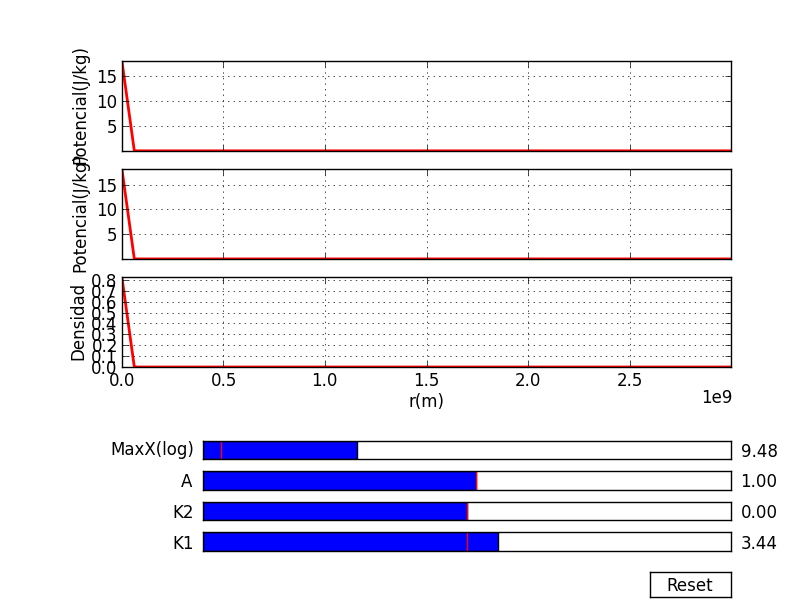
\includegraphics[scale=0.7]{potencial1.png}
 \caption{\emph{Potencial A = 1, rango del radio hasta 3*10**9}}
 \label{Fig: 1}
\end{figure}

\begin{figure}[!h]
 \centering
 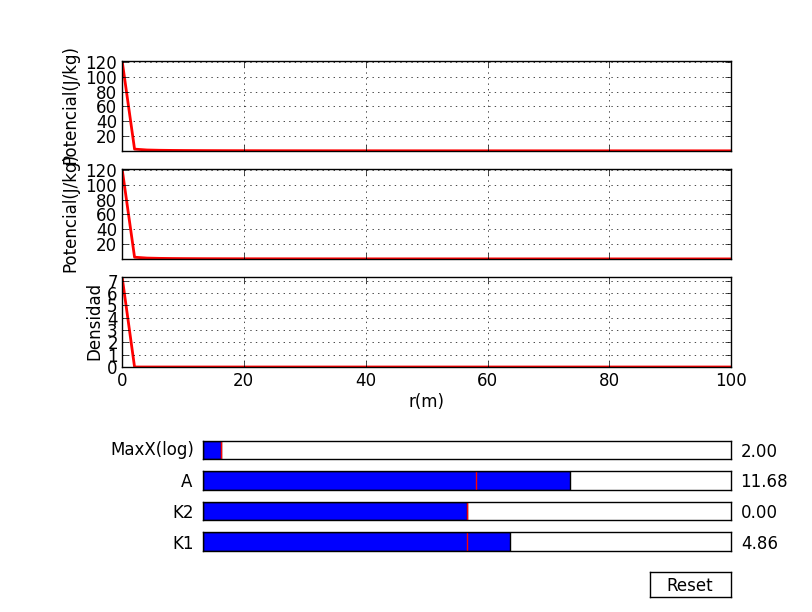
\includegraphics[scale=0.7]{potencial3.png}
 \caption{\emph{Potencial A mayor que 1}}
 \label{Fig: 3}
\end{figure}

\begin{figure}[!h]
 \centering
 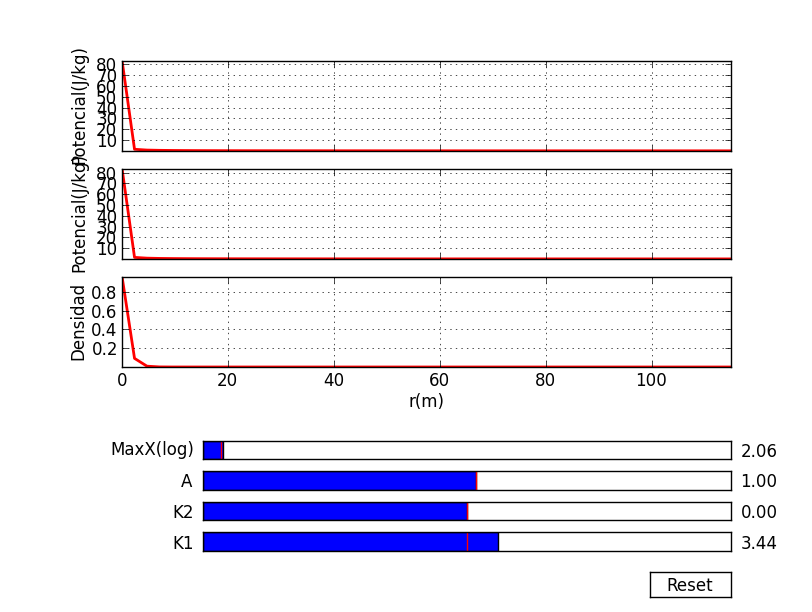
\includegraphics[scale=0.7]{potencial2.png}
 \caption{\emph{Potencial A = 1}}
 \label{Fig: 2}
\end{figure}


\begin{figure}[!h]
 \centering
 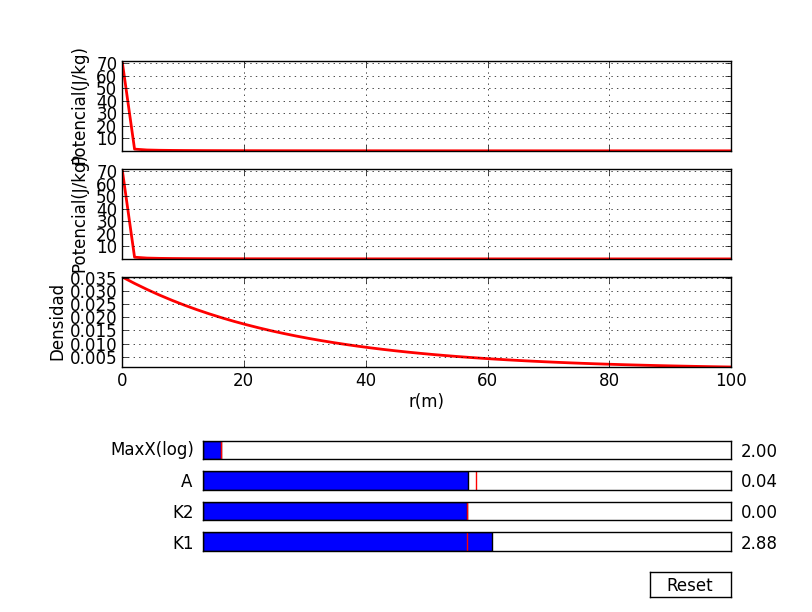
\includegraphics[scale=0.7]{potencial4.png}
 \caption{\emph{Potencial A in (0,1) }}
 \label{Fig: 1}
\end{figure}


\begin{figure}[!h]
 \centering
 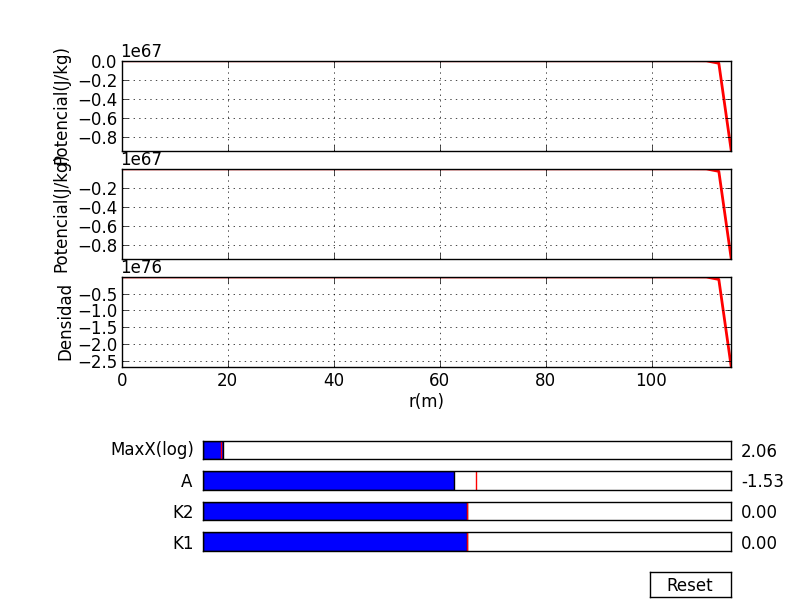
\includegraphics[scale=0.7]{potencial5.png}
 \caption{\emph{Potencial  A menor que 0}}
 \label{Fig: 1}
\end{figure}

\begin{figure}[!h]
 \centering
 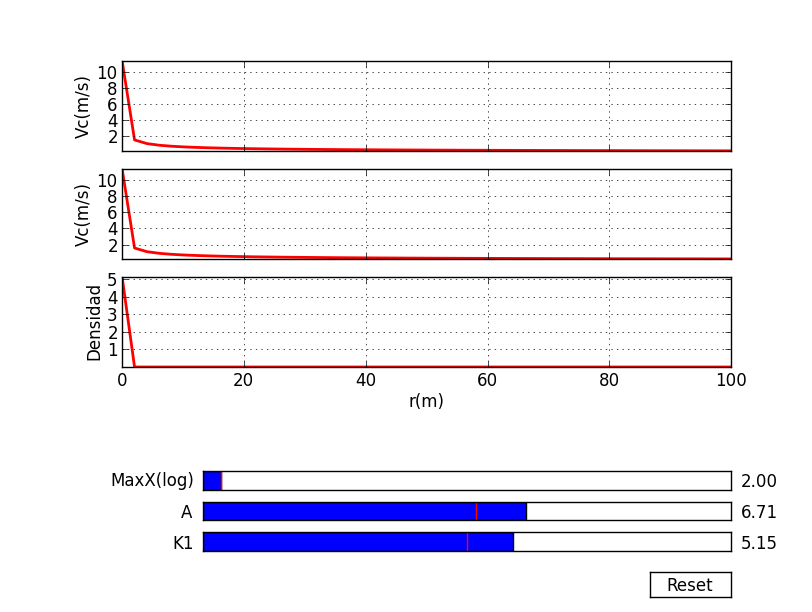
\includegraphics[scale=0.7]{velocity4.png}
 \caption{\emph{Vc A mayor que 1}}
 \label{Fig: 1}
\end{figure}

\begin{figure}[!h]
 \centering
 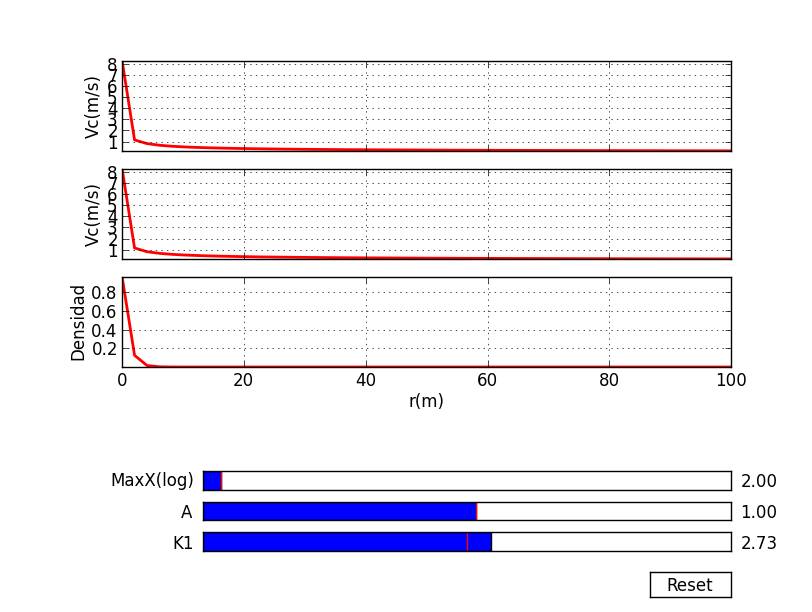
\includegraphics[scale=0.7]{velocity.png}
 \caption{\emph{Velocidad A = 1}}
 \label{Fig: 1}
\end{figure}

\begin{figure}[!h]
 \centering
 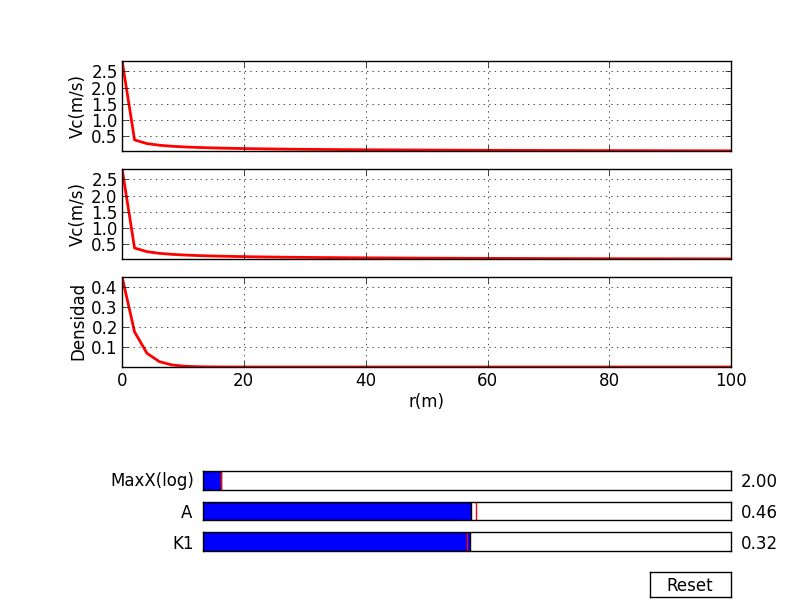
\includegraphics[scale=0.7]{velocity2.png}
 \caption{\emph{Vc A in (0,1) }}
 \label{Fig: 1}
\end{figure}

\begin{figure}[!h]
 \centering
 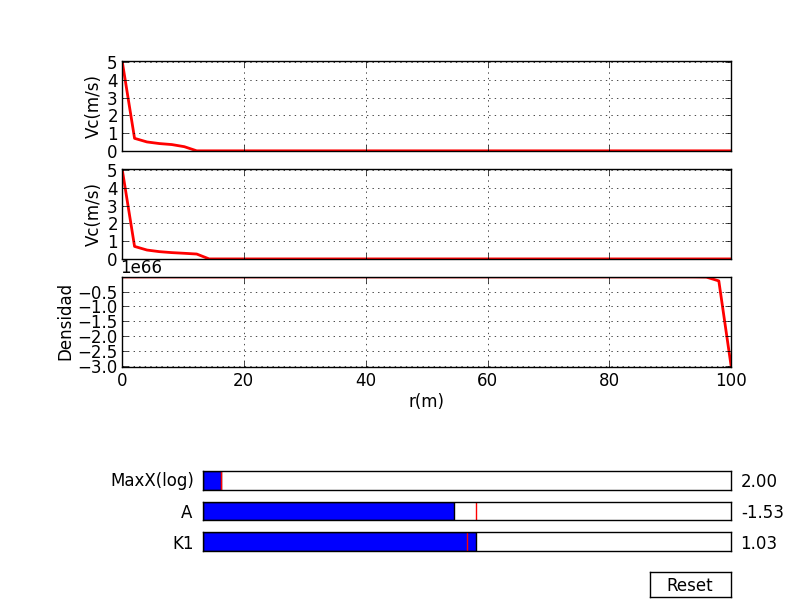
\includegraphics[scale=0.7]{velocity3.png}
 \caption{\emph{Velocidad circular A menor que 0}}
 \label{Fig: 1}
\end{figure}



\begin{figure}[!h]
 \centering
 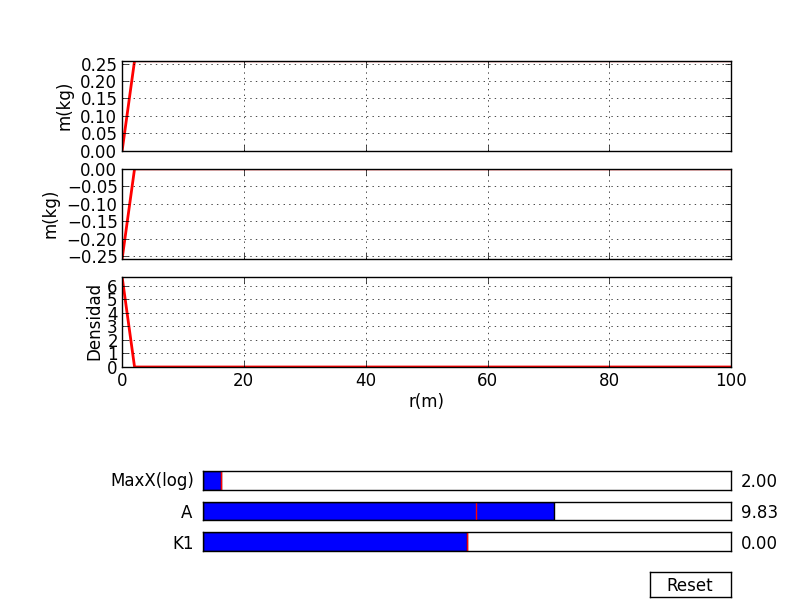
\includegraphics[scale=0.7]{masa4.png}
 \caption{\emph{Masa mayor que 1 }}
 \label{Fig: 1}
\end{figure}


\begin{figure}[!h]
 \centering
 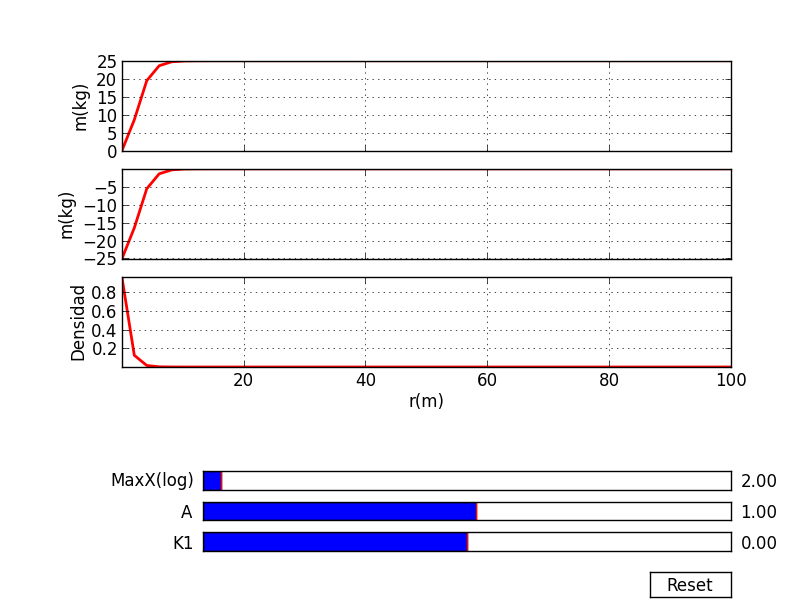
\includegraphics[scale=0.7]{masa1.png}
 \caption{\emph{Masa A = 1}}
 \label{Fig: 1}
\end{figure}

\begin{figure}[!h]
 \centering
 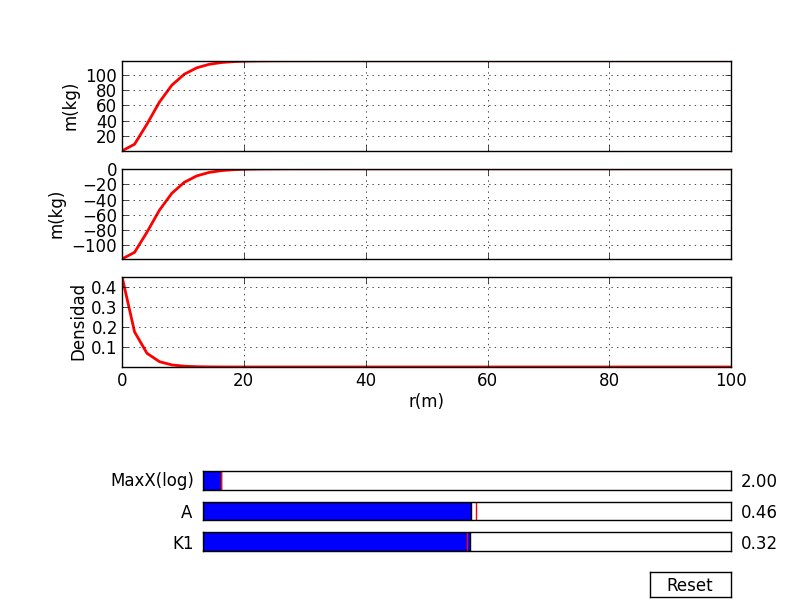
\includegraphics[scale=0.7]{masa2.png}
 \caption{\emph{Masa A in (0,1) }}
 \label{Fig: 1}
\end{figure}


\begin{figure}[!h]
 \centering
 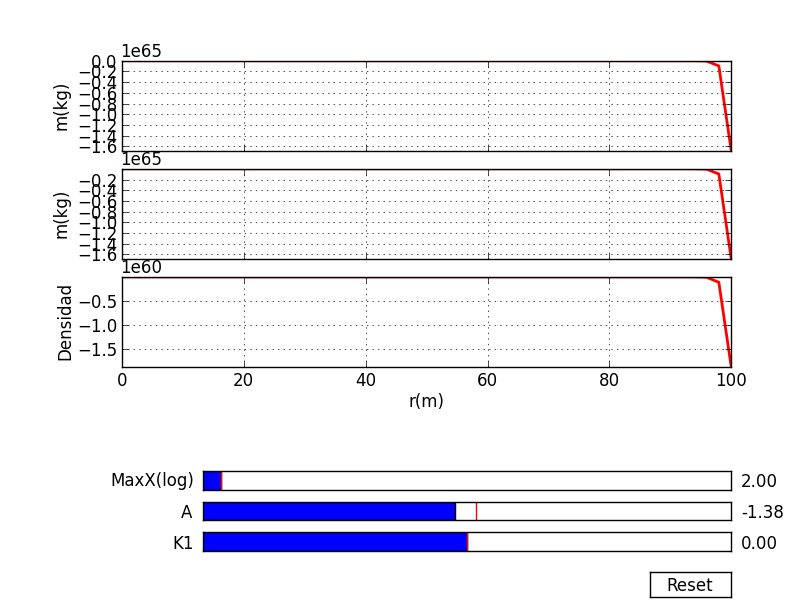
\includegraphics[scale=0.7]{masa3.png}
 \caption{\emph{Masa A menor que 0}}
 \label{Fig: 1}
\end{figure}



\begin{figure}[!h]
 \centering
 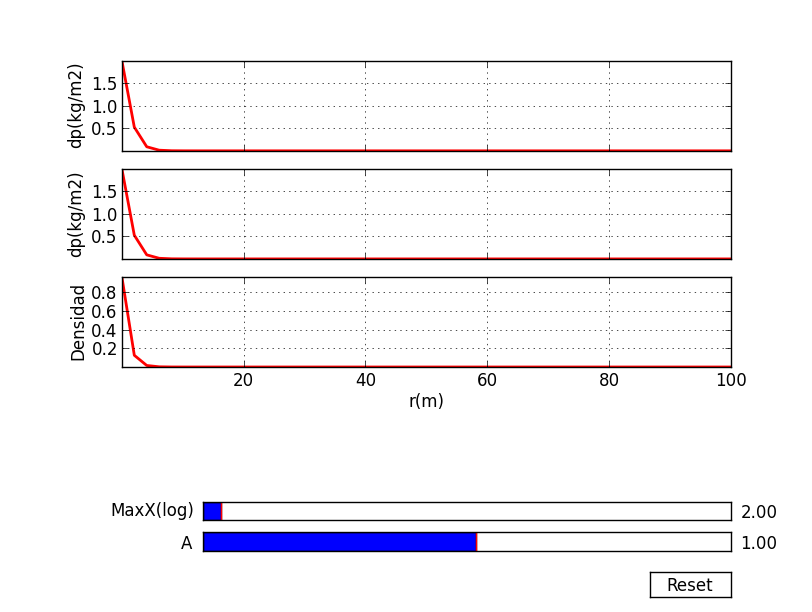
\includegraphics[scale=0.7]{dp1.png}
 \caption{\emph{Distribución proyectada A = 1}}
 \label{Fig: 1}
\end{figure}


\begin{figure}[!h]
 \centering
 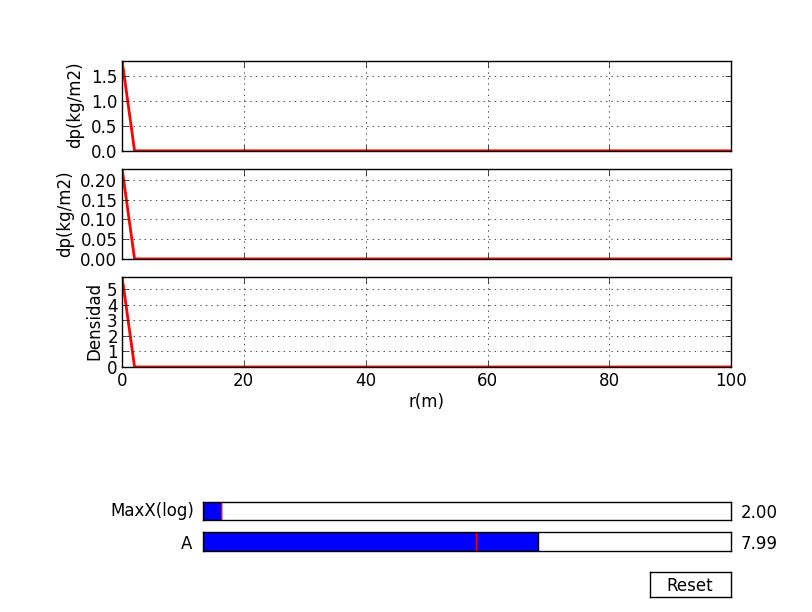
\includegraphics[scale=0.7]{dp2.png}
 \caption{\emph{Distribución proyectada A mayor que 1}}
 \label{Fig: 1}
\end{figure}

\begin{figure}[!h]
 \centering
 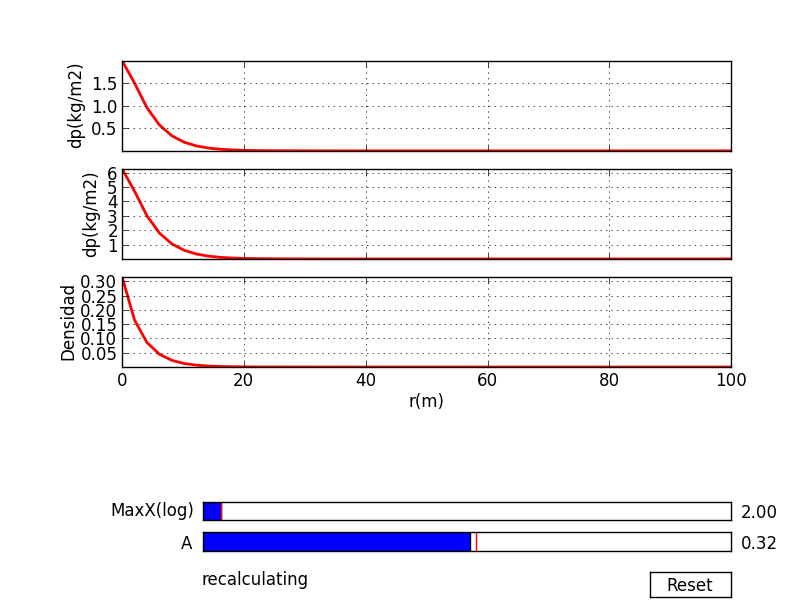
\includegraphics[scale=0.7]{dp3.png}
 \caption{\emph{Distribucion proyectada A in (0,1) }}
 \label{Fig: 1}
\end{figure}



\end{document}

